\chapter{Evaluation}

This chapter evaluates the system against the three research questions.
Section 5.1 describes the experimental setup shared by all experiments.
Section 5.2 addresses RQ1 by comparing multi-modal retrieval against a
text-only baseline. Section 5.3 addresses RQ2 through a series of
ablations over the embedding and retrieval strategy --- modality fusion,
query decomposition, second-stage re-ranking, and the embedding backbone
--- including two negative results that shaped the final design. Section
5.4 addresses RQ3 by measuring end-to-end question-answering accuracy of
the agentic pipeline, culminating in a controlled experiment that
isolates the contribution of visual evidence at the answering stage.
Section 5.5 replicates the modality comparison on a speech-dense second
domain (YouCook2), testing the domain-conditionality prediction that
Chapter 6 attaches to the text-channel negative results. Section 5.6
reports system-level costs. Every number in this chapter is reproducible
from the committed result files (\texttt{results/*.json}); the exact
command that produced each result is recorded in
\texttt{docs/EXPERIMENTS.md}.

\section{Experimental setup}

\textbf{Dataset.} All experiments use the validation split of NExT-QA
\autocite{xiao2021nextqa}, a benchmark of causal and temporal
multiple-choice questions over short (\textasciitilde44 s) everyday
videos, together with the temporal grounding labels contributed by
NExT-GQA \autocite{xiao2024nextgqa}. The split contains 3,358 questions
over 567 videos, and --- after intersecting with the grounding
annotations --- every question carries at least one ground-truth
temporal interval locating the evidence for its answer. NExT-GQA was
chosen over larger retrieval benchmarks (e.g.~MSRVTT, ActivityNet
Captions) precisely because these interval labels allow retrieval to be
scored with \emph{temporal} precision rather than at whole-video
granularity.

\textbf{Indexing.} The ingestion pipeline of Chapter 3 produced 5,725
overlapping segments (8 s window, 4 s stride) from the 567 videos. Each
segment is indexed in two ChromaDB collections (HNSW, cosine): a visual
collection holding the pooled CLIP embedding of the segment's keyframes
(5,725 vectors), and a text collection holding the CLIP text embedding
of its speech transcript (3,433 vectors --- 60\% of segments contain
speech). Unless stated otherwise the index backbone is CLIP ViT-B-32
(laion2b); Section 5.3.4 varies the backbone.

\textbf{Retrieval metrics.} For each question, the question text is used
as the query and the top-K segments are retrieved. A retrieved segment
counts as a \emph{hit} if it comes from the ground-truth video
\textbf{and} its temporal interval overlaps a ground-truth interval with
tIoU ≥ τ; requiring both conditions ties the metric to moment-level
retrieval rather than video identification. Reported metrics are
Recall@\{1,5,10\} and MRR at the primary threshold τ = 0.5, nDCG@10 with
graded tIoU gains (ideal-normalised against the ground-truth video's own
segments), and tIoU@1 --- the mean temporal overlap of the top-ranked
segment, the dissertation's ``temporal accuracy'' measure. Section 5.3.5
repeats key configurations at the looser τ = 0.3.

\textbf{Scopes.} Two retrieval scopes are evaluated. In \textbf{corpus}
scope the query searches all 5,725 segments across 567 videos --- the
full RQ1 setting, where the system must find both the right video and
the right moment. In \textbf{video} scope the search is restricted to
the ground-truth video's own segments, isolating pure temporal
localisation. The gap between the two scopes attributes error to
cross-video confusion versus within-video imprecision.

\textbf{QA metric.} Section 5.4 evaluates answer generation directly on
NExT-QA's five-way multiple-choice format: the agent receives the
question and its five options, gathers evidence with its tools, and must
emit a final option index. Accuracy is reported overall and per question
type (CW/CH: causal \emph{why}/\emph{how}; TN/TC/TP: temporal
\emph{next}/\emph{current}/\emph{previous}). The random-guess floor is
0.20.

\textbf{Implementation constants.} Unless varied by the ablation, fusion
weight α = 0.5, retrieval depth K = 10, re-ranker candidate pool 30, and
the question encoder matches the index backbone. All retrieval
experiments are deterministic given the committed decomposition cache;
agent experiments use temperature-default API calls and are therefore
subject to normal LLM variance.

\section{RQ1 --- Multi-modal retrieval against a text-only
baseline}

Table 5.1 reports the three single-strategy configurations on both
scopes at τ = 0.5. The text-only baseline embeds each segment's Whisper
transcript and searches it with the question text --- the standard
``search what was said'' approach that RQ1 asks the system to beat. A
reminder of scale before reading the table (§1.2): a hit requires the
correct video \emph{and} tIoU ≥ 0.5 between an 8-second window and the
annotated moment, searched over all 5,725 segments --- a deliberately
strict criterion under which absolute scores are small by construction,
so the informative content of the table is in the \emph{relative}
comparisons between rows, not in the magnitudes.

\textbf{Table 5.1 --- Retrieval by modality (ViT-B-32 index, τ = 0.5).}

\begin{longtable}[]{@{}llllllll@{}}
\toprule\noalign{}
Scope & Modality & R@1 & R@5 & R@10 & MRR & nDCG@10 & tIoU@1 \\
\midrule\noalign{}
\endhead
\bottomrule\noalign{}
\endlastfoot
corpus & visual & .026 & .075 & .111 & .047 & .117 & .035 \\
corpus & text & .002 & .005 & .011 & .004 & .011 & .003 \\
corpus & fused (α=.5) & .002 & .010 & .013 & .005 & .018 & .007 \\
video & visual & .148 & .394 & .491 & .250 & .659 & .203 \\
video & text & .080 & .232 & .305 & .143 & .390 & .117 \\
video & fused (α=.5) & .129 & .384 & .491 & .235 & .639 & .186 \\
\end{longtable}

Three observations answer RQ1. First, \emph{visual retrieval dominates
text retrieval by an order of magnitude in corpus scope} (R@10 .111 vs
.011): to find a moment among 567 videos of everyday footage, what is
\emph{on screen} is far more discriminative than what is \emph{said}.
Second, two causes plausibly account for the failure of the text
channel, and neither is poor transcription as such. NExT-QA's home
videos contain sparse, conversational, and frequently non-English speech
(German, Mandarin and other languages appear in the transcripts), so the
information a question asks about is often simply \emph{absent} from the
speech --- a question about what a child \emph{does} is rarely answered
by what anyone \emph{says}. And the CLIP text encoder that embeds both
queries and transcripts is trained predominantly on English alt-text, so
even present information may be \emph{unreadable} to it. These two
causes are entangled in this experiment; §6.2 explains why the present
design cannot apportion blame between them, and names the
translate-then-embed variant that would. Third, the corpus/video gap
localises the difficulty: within the correct video the system already
ranks a correct moment in its top five for 39\% of questions, but across
the corpus R@10 falls to 11\% --- \emph{cross-video confusion, not
within-video imprecision, is the dominant error mode}, which motivates
the precision-oriented interventions of Section 5.3.

The by-type breakdown (Appendix B) shows temporal-precise question types
(TP, n = 52) retrieving worst in corpus scope, previewing the
temporal-reasoning theme of Section 5.4.

\section{RQ2 --- Embedding and retrieval strategy
ablations}

\subsection{Negative result: naive late fusion never beats
visual-only}

The natural response to a weak-but-nonzero text channel is weighted late
fusion: score = α·visual + (1−α)·text. Figure 5.1 sweeps α over \{0.5,
0.7, 0.8, 0.9\} in corpus scope. Every metric rises monotonically toward
the α = 1.0 endpoint --- visual-only --- and none crosses it; the same
holds in video scope, where the best fused configuration (α = 0.8) ties
visual-only on R@10 (.494 vs .491) but loses on R@1 (.139 vs .148) and
MRR (.244 vs .250). At α = 0.5 fusion is catastrophic in corpus scope
(R@10 .013) because the text scores act as high-variance noise added to
a weak-but-real visual signal.

\begin{figure}
\centering
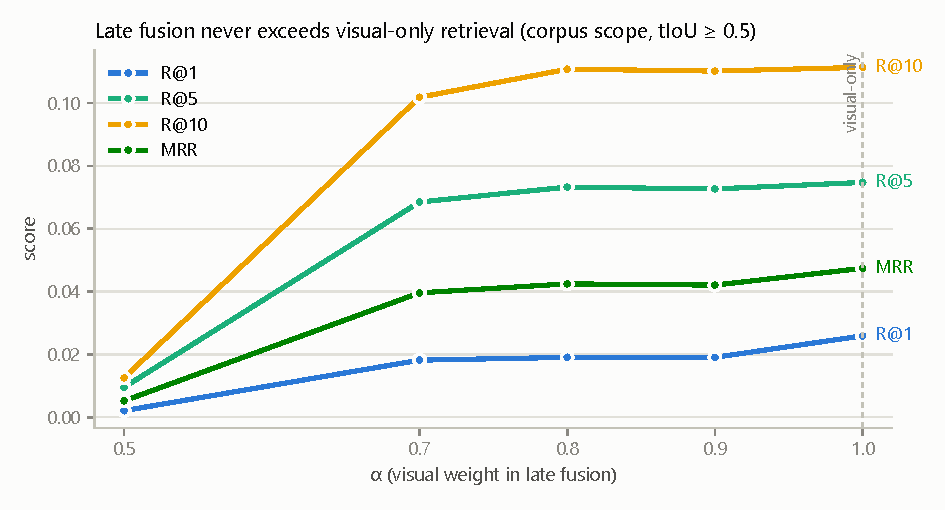
\includegraphics[width=0.82\linewidth,height=\textheight,keepaspectratio,alt={Late-fusion weight sweep in corpus scope.}]{../figures/fig4_alpha_sweep.pdf}
\caption{Late-fusion weight sweep in corpus
scope.}
\end{figure}

The conclusion is sharper than ``tune α'': \emph{with this text channel,
there is no fusion weight at which the transcript embeddings contribute
positive evidence.} Fusion is not a weighting problem but a
channel-quality problem --- the actionable implication being to repair
the text channel (e.g.~translate transcripts to English before
embedding, or use a dedicated multilingual text-retrieval encoder)
before re-introducing it, rather than to search the weight space
further. All subsequent experiments therefore use the visual modality.

\subsection{Query decomposition recalls more, but no more
precisely}

NExT-QA questions are causal and temporal (``why did the boy pick up one
present from the group of them and move to the sofa''), whereas CLIP
matches literal scene descriptions. The W5 decomposer prompts an LLM to
rewrite each question into at most four short scene captions (``a boy
picks up a present from a group of presents'', ``a boy carries a present
and walks to a sofa'', \ldots), retrieves each caption plus the original
question independently, and fuses the rankings with reciprocal rank
fusion. The rewrite is computed once per question and cached (3,358
questions approximately US\$0.15 of LLM usage).

Decomposition lifts the deep-rank metrics in corpus scope --- R@10 .111
\ensuremath{\rightarrow} .122 (+9.9\% relative), R@5 +6.7\%, MRR +6.4\%
--- while leaving the top of the ranking essentially untouched (R@1 .026
\ensuremath{\rightarrow} .025, tIoU@1 unchanged at .035; Table 5.2, rows
1--2; Figure 5.2). The pattern is informative: translating abstract
questions into CLIP-native captions surfaces \emph{additional correct
candidates} into the top ten, but rank fusion of near-tied cosine scores
cannot push them to position one. Recall problems and precision problems
are separable; decomposition solves a recall problem, and the next
section supplies the missing precision.

\subsection{Second-stage re-ranking: a negative and a positive
result}

\textbf{Text cross-encoder (negative).} The project plan anticipated a
standard text cross-encoder re-ranker (bge-reranker) scoring (question,
transcript) pairs over the candidate pool. On a 100-question development
subset this \emph{reduced} quality at every fusion weight tested --- at
weight 0.5 it halved R@5 (.070 \ensuremath{\rightarrow} .030), and even
at 0.8 it remained below the no-reranking baseline. One asymmetry should
be stated plainly: this negative result rests on 100 questions, whereas
every positive retrieval result in this chapter is measured on all
3,358. The component was rejected on the development subset and never
promoted to a full-split run, so the evidence against it is weaker than
the evidence for the components that replaced it --- a decision
revisited in §6.3. The mechanism mirrors §5.3.1: the transcripts are
conversational chatter, largely uncorrelated with the visual events the
questions ask about, so every reordering the cross-encoder makes injects
noise. An implementation subtlety compounds the problem and is worth
recording: 40\% of segments have no transcript at all, and if such
candidates simply receive no re-ranker score, any scored candidate the
cross-encoder likes outranks \emph{every} unscored one --- structurally
demoting exactly the visual-only segments most likely to be correct.
(The first implementation here had this flaw, and drove R@1 to zero.)
The repaired design imputes the re-ranker term of a modality-missing
candidate from its retrieval rank, keeping both candidate classes on one
score scale; the negative result above is reported \emph{with} this
repair, so it reflects the channel, not the bug.

\textbf{Visual re-ranker (positive).} The replacement re-ranker
re-scores the top-30 candidates with a stronger vision model (CLIP
ViT-L-14) over pre-computed segment embeddings, fusing the ViT-L ranking
with the first-stage ranking by weighted RRF. Every segment has
keyframes, so the missing-modality problem vanishes. Table 5.2 and
Figure 5.2 show the ladder at τ = 0.5, corpus scope:

\begin{figure}
\centering
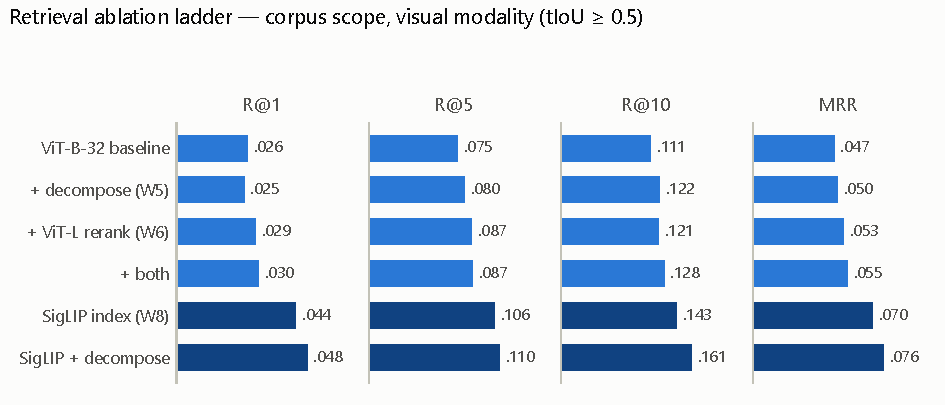
\includegraphics[width=0.86\linewidth,height=\textheight,keepaspectratio,alt={Retrieval ablation ladder from the baseline to the final configuration.}]{../figures/fig5_ablation_ladder.pdf}
\caption{Retrieval ablation ladder from the baseline to the final
configuration.}
\end{figure}

\textbf{Table 5.2 --- Corpus-scope ablation ladder (visual modality, τ =
0.5).}

\begin{longtable}[]{@{}
  >{\raggedright\arraybackslash}p{(\linewidth - 10\tabcolsep) * \real{0.1667}}
  >{\raggedright\arraybackslash}p{(\linewidth - 10\tabcolsep) * \real{0.1667}}
  >{\raggedright\arraybackslash}p{(\linewidth - 10\tabcolsep) * \real{0.1667}}
  >{\raggedright\arraybackslash}p{(\linewidth - 10\tabcolsep) * \real{0.1667}}
  >{\raggedright\arraybackslash}p{(\linewidth - 10\tabcolsep) * \real{0.1667}}
  >{\raggedright\arraybackslash}p{(\linewidth - 10\tabcolsep) * \real{0.1667}}@{}}
\toprule\noalign{}
\begin{minipage}[b]{\linewidth}\raggedright
Configuration
\end{minipage} & \begin{minipage}[b]{\linewidth}\raggedright
R@1
\end{minipage} & \begin{minipage}[b]{\linewidth}\raggedright
R@5
\end{minipage} & \begin{minipage}[b]{\linewidth}\raggedright
R@10
\end{minipage} & \begin{minipage}[b]{\linewidth}\raggedright
MRR
\end{minipage} & \begin{minipage}[b]{\linewidth}\raggedright
tIoU@1
\end{minipage} \\
\midrule\noalign{}
\endhead
\bottomrule\noalign{}
\endlastfoot
ViT-B-32 baseline & .026 & .075 & .111 & .047 & .035 \\
+ decomposition (W5) & .025 & .080 & .122 & .050 & .035 \\
+ ViT-L re-ranking (W6) & .029 & .087 & .121 & .053 & .041 \\
+ both & .030 & .087 & .128 & .055 & .040 \\
SigLIP index (W8) & .044 & .106 & .143 & .070 & .054 \\
SigLIP + decomposition & \textbf{.048} & \textbf{.110} & \textbf{.161} &
\textbf{.076} & .055 \\
\end{longtable}

The two mid-pipeline interventions compose additively: decomposition
contributes at depth, re-ranking at the top of the list, and their
combination improves every metric over the baseline (+15--17\% relative
on MRR and R@10). In video scope the combined configuration reaches R@1
.154, R@10 .501, tIoU@1 .209 --- each the best of any ViT-B
configuration.

\subsection{Backbone: SigLIP dominates, and two-stage retrieval matches
one-stage}

The final RQ2 axis exchanges the embedding backbone itself, holding
segmentation and evaluation fixed. Three backbones were compared as
\emph{the index}: CLIP ViT-B-32 (baseline), CLIP ViT-L-14, and SigLIP
SO400M (webli), each with its own question encoder.

Two findings emerge from Table 5.2 (bottom rows) and Table 5.3. First,
\emph{SigLIP is categorically stronger for this task}: as the index it
lifts corpus R@1 by 69\% relative over ViT-B (.026
\ensuremath{\rightarrow} .044) and tIoU@1 by 54\%, and with
decomposition on top reaches R@1 .048 --- \emph{nearly double the
original baseline} --- and video-scope tIoU@1 .230. This is consistent
with SigLIP's sigmoid-loss pretraining, which has been reported to
favour retrieval tasks \autocite{zhai2023siglip}.

Second, ViT-L used as the full index (corpus R@1 .029, R@5 .090, R@10
.122, MRR .054) is indistinguishable at the resolution of this
evaluation from ViT-B \emph{plus} ViT-L re-ranking (.029/.087/.121/.053)
--- every metric agrees to within ±.003, though the pair was compared
numerically and not by a significance test. \emph{The two-stage
cheap-index/expensive-re-ranker design recovers essentially all of the
larger model's quality} while embedding the corpus only with the small
model; at larger corpus scales, where re-embedding everything with the
expensive model is prohibitive, the two-stage design is the scalable
route to the same accuracy. A corollary worth stating for practitioners:
a re-ranker must \emph{differ} from the index model --- re-scoring with
the index's own embeddings is an identity operation.

\textbf{Table 5.3 --- Video-scope backbone comparison (visual modality,
τ = 0.5).}

\begin{longtable}[]{@{}
  >{\raggedright\arraybackslash}p{(\linewidth - 10\tabcolsep) * \real{0.1667}}
  >{\raggedright\arraybackslash}p{(\linewidth - 10\tabcolsep) * \real{0.1667}}
  >{\raggedright\arraybackslash}p{(\linewidth - 10\tabcolsep) * \real{0.1667}}
  >{\raggedright\arraybackslash}p{(\linewidth - 10\tabcolsep) * \real{0.1667}}
  >{\raggedright\arraybackslash}p{(\linewidth - 10\tabcolsep) * \real{0.1667}}
  >{\raggedright\arraybackslash}p{(\linewidth - 10\tabcolsep) * \real{0.1667}}@{}}
\toprule\noalign{}
\begin{minipage}[b]{\linewidth}\raggedright
Index backbone
\end{minipage} & \begin{minipage}[b]{\linewidth}\raggedright
R@1
\end{minipage} & \begin{minipage}[b]{\linewidth}\raggedright
R@5
\end{minipage} & \begin{minipage}[b]{\linewidth}\raggedright
R@10
\end{minipage} & \begin{minipage}[b]{\linewidth}\raggedright
MRR
\end{minipage} & \begin{minipage}[b]{\linewidth}\raggedright
tIoU@1
\end{minipage} \\
\midrule\noalign{}
\endhead
\bottomrule\noalign{}
\endlastfoot
ViT-B-32 & .148 & .394 & .491 & .250 & .203 \\
ViT-L-14 & .151 & .407 & .496 & .257 & .210 \\
SigLIP SO400M & .170 & .406 & .494 & .266 & .221 \\
SigLIP + decomposition & \textbf{.176} & \textbf{.419} & \textbf{.496} &
\textbf{.275} & \textbf{.230} \\
\end{longtable}

\subsection{Threshold sensitivity}

τ = 0.5 is a strict criterion for 8-second windows scored against
ground-truth intervals of arbitrary length. Table 5.4 repeats the ViT-B
baseline and the best ViT-B configuration at τ = 0.3; the binary metrics
roughly double, while tIoU@1, which is threshold-free, is unchanged by
construction.

\textbf{Table 5.4 --- Threshold sensitivity (visual modality, ViT-B
index).}

\begin{longtable}[]{@{}lllllll@{}}
\toprule\noalign{}
Scope & Configuration & τ & R@1 & R@5 & R@10 & MRR \\
\midrule\noalign{}
\endhead
\bottomrule\noalign{}
\endlastfoot
corpus & baseline & 0.5 & .026 & .075 & .111 & .047 \\
corpus & baseline & 0.3 & .054 & .130 & .186 & .089 \\
corpus & + decompose + rerank & 0.5 & .030 & .087 & .128 & .055 \\
corpus & + decompose + rerank & 0.3 & .062 & .151 & .208 & .101 \\
video & baseline & 0.5 & .148 & .394 & .491 & .250 \\
video & baseline & 0.3 & .311 & .660 & .774 & .456 \\
video & + decompose + rerank & 0.5 & .154 & .410 & .501 & .258 \\
video & + decompose + rerank & 0.3 & .323 & .677 & .780 & .469 \\
\end{longtable}

Two conclusions follow: the system's practical localisation ability
(``lands within a loose overlap of the right moment'') is considerably
better than the strict headline numbers suggest --- within the correct
video, a correct moment is in the top five for two-thirds of questions
--- and the relative ordering of configurations is stable across
thresholds, so the ablation conclusions above do not depend on the
choice of τ.

\section{RQ3 --- Agentic question
answering}

\subsection{Agent comparison}

Table 5.5 and Figure 5.3 compare the two agent designs of Chapter 3 on
the first 150 grounded val questions under a text-only LLM
(deepseek-chat \autocite{deepseek2024v3}): the single-loop
function-calling agent (W4) and the LangGraph state machine (W7), which
adds the temporal tool (\texttt{get\_segments\_around}) and a bounded
self-reflection pass that audits the draft answer's citations against
the gathered evidence before accepting it.

\begin{figure}
\centering
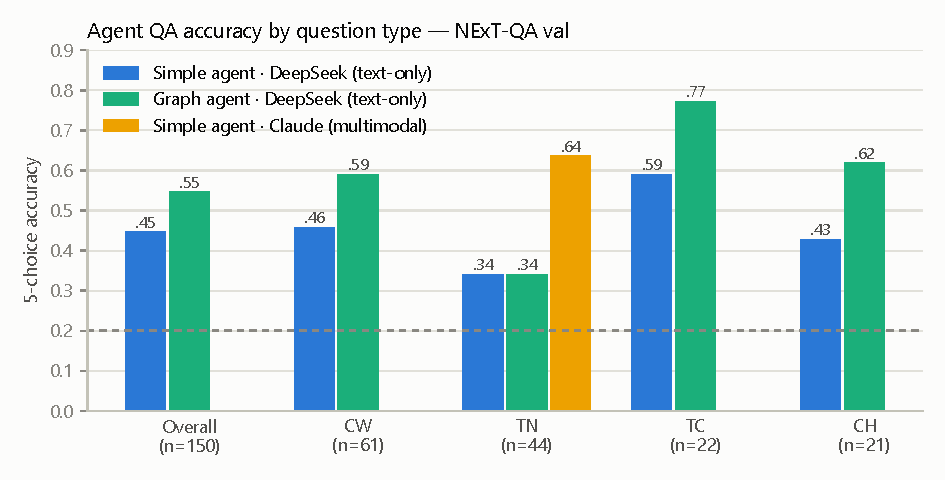
\includegraphics[width=0.88\linewidth,height=\textheight,keepaspectratio,alt={Question-answering accuracy by question type and agent configuration.}]{../figures/fig7_qa_by_type.pdf}
\caption{Question-answering accuracy by question type and agent
configuration.}
\end{figure}

\textbf{Table 5.5 --- Five-choice QA accuracy, 150 val questions.} Three
variables move across these rows --- agent, base model, and evidence
channel --- so only rows sharing two of the three are directly
comparable; §5.4.3 draws the valid pairings. TP is omitted from the
by-type columns (n = 2) and reported in Appendix B.

\begin{longtable}[]{@{}
  >{\raggedright\arraybackslash}p{(\linewidth - 14\tabcolsep) * \real{0.1250}}
  >{\raggedright\arraybackslash}p{(\linewidth - 14\tabcolsep) * \real{0.1250}}
  >{\raggedright\arraybackslash}p{(\linewidth - 14\tabcolsep) * \real{0.1250}}
  >{\raggedright\arraybackslash}p{(\linewidth - 14\tabcolsep) * \real{0.1250}}
  >{\raggedright\arraybackslash}p{(\linewidth - 14\tabcolsep) * \real{0.1250}}
  >{\raggedright\arraybackslash}p{(\linewidth - 14\tabcolsep) * \real{0.1250}}
  >{\raggedright\arraybackslash}p{(\linewidth - 14\tabcolsep) * \real{0.1250}}
  >{\raggedright\arraybackslash}p{(\linewidth - 14\tabcolsep) * \real{0.1250}}@{}}
\toprule\noalign{}
\begin{minipage}[b]{\linewidth}\raggedright
Agent
\end{minipage} & \begin{minipage}[b]{\linewidth}\raggedright
Base model
\end{minipage} & \begin{minipage}[b]{\linewidth}\raggedright
Evidence
\end{minipage} & \begin{minipage}[b]{\linewidth}\raggedright
Overall
\end{minipage} & \begin{minipage}[b]{\linewidth}\raggedright
CW (n=61)
\end{minipage} & \begin{minipage}[b]{\linewidth}\raggedright
TN (n=44)
\end{minipage} & \begin{minipage}[b]{\linewidth}\raggedright
TC (n=22)
\end{minipage} & \begin{minipage}[b]{\linewidth}\raggedright
CH (n=21)
\end{minipage} \\
\midrule\noalign{}
\endhead
\bottomrule\noalign{}
\endlastfoot
Simple loop (W4) & deepseek-chat & text-only & .447 & .459 & .341 & .591
& .429 \\
LangGraph (W7) & deepseek-chat & text-only & .547 & .590 & .341 & .773 &
.619 \\
none --- prior only (§5.4.3) & deepseek-chat & none & .560 & .574 & .568
& .545 & .524 \\
none --- prior only (§5.4.3) & claude-opus-4-8 & none & .560 & .639 &
.455 & .591 & .476 \\
LangGraph (W7), best config (§5.4.4) & claude-opus-4-8 & multimodal &
\textbf{.727} & \textbf{.852} & .568 & .682 & \textbf{.762} \\
\end{longtable}

Both agents clear the .20 random floor by a wide margin --- although
§5.4.3 will show that the random floor is the wrong bar, since the bare
model answers at .560 with no evidence at all; the informative
comparison in this section is between the two agents, which saw
identical evidence. The graph agent improves overall accuracy by 10
points (+22\% relative), with the gains concentrated in causal questions
(CW +13.1, CH +19.0 points) and temporal-current questions (TC +18.2).
Because both agents answered the identical 150 questions, the comparison
is paired: 29 questions flipped to correct under the graph agent against
14 that flipped to incorrect, giving an exact McNemar p = .031, with a
paired-bootstrap 95\% CI on the difference of {[}+.013, +.187{]} (10,000
resamples) --- the improvement is unlikely to be run-to-run LLM
variance. Inspection of transcripts attributes the gains to three
behaviours: systematic anchor-then-walk retrieval on temporal questions,
reformulated follow-up searches when initial evidence is thin, and the
reflection pass --- which in observed runs rejected drafts whose
citations did not appear in the gathered evidence, forcing a grounded
rewrite.

The striking exception is TN (\emph{what happened next}), frozen at .341
for \textbf{both} agents. Qualitative inspection shows the temporal
machinery working exactly as designed --- the agent anchors the cue
event and retrieves the segments that follow it --- and then failing at
the last step: the answer to a TN question is almost always a
\emph{visual action} (what a person or animal does next), the following
segments are typically silent, and a text-only LLM receives no usable
evidence. In one representative case (``what does the white dog do after
going to the cushion'', ground truth \emph{smells the black dog}), the
text-only agent responded that the post-anchor segments contain no
speech and the action ``cannot be determined from the available
evidence'' --- a correct description of its own evidence starvation.

\subsection{Controlled experiment: visual evidence at the answering
stage}

The TN result yields a precise hypothesis: the bottleneck is the
\emph{evidence channel}, not the temporal mechanism. To test it, the
same 44 TN questions were re-run under the \emph{simple} agent with a
single change from its own text-only row: the provider was switched to a
multimodal LLM (claude-opus-4-8), whose tool results embed each
segment's keyframe image alongside the transcript. Retrieval index,
tools, prompts, and questions were held fixed. The agent is named
because it matters for the comparison: the LangGraph harness targeted
OpenAI-compatible providers only at the time of this experiment, so the
strict single-variable contrast is row 1 against row 3 of Table 5.6. The
graph-agent row is listed because it lands on the identical .341, which
makes the same conclusion hold against it; the graph-plus-multimodal
combination was implemented later and is evaluated in §5.4.4.

\textbf{Table 5.6 --- Same 44 TN questions, evidence channel varied.}

\begin{longtable}[]{@{}ll@{}}
\toprule\noalign{}
Configuration & TN accuracy \\
\midrule\noalign{}
\endhead
\bottomrule\noalign{}
\endlastfoot
Text-only LLM, simple agent & .341 \\
Text-only LLM, graph agent (temporal tool) & .341 \\
\textbf{Multimodal LLM, simple agent, keyframes in evidence} &
\textbf{.636} \\
\end{longtable}

Accuracy rises by 29.5 points (+87\% relative, 44/44 questions
completed). This comparison is likewise paired on identical questions:
against the graph agent, 16 questions flipped to correct under visual
evidence and 3 flipped away (exact McNemar p = .004; paired-bootstrap
95\% CI {[}+.114, +.455{]}; against the simple agent, p = .007). On the
representative case above, the multimodal agent answered ``leans down
and sniffs/nuzzles the small black puppy {[}28--36 s{]}'' --- matching
the ground truth almost verbatim from the keyframes alone; Figure 5.4
shows the keyframes in question beside the two models' verbatim answers.
Because everything except the evidence modality was held constant, the
improvement is attributable to visual evidence at the answering stage;
§5.4.3 adds the absolute calibration --- .636 also clears the multimodal
model's own no-evidence prior on TN (.455) by +.18. Together with
Section 5.2, this closes the loop on the modality question at
\emph{both} ends of the pipeline: retrieval needs visual embeddings to
find the right moment, and generation needs visual evidence to describe
it.

\begin{figure}
\centering
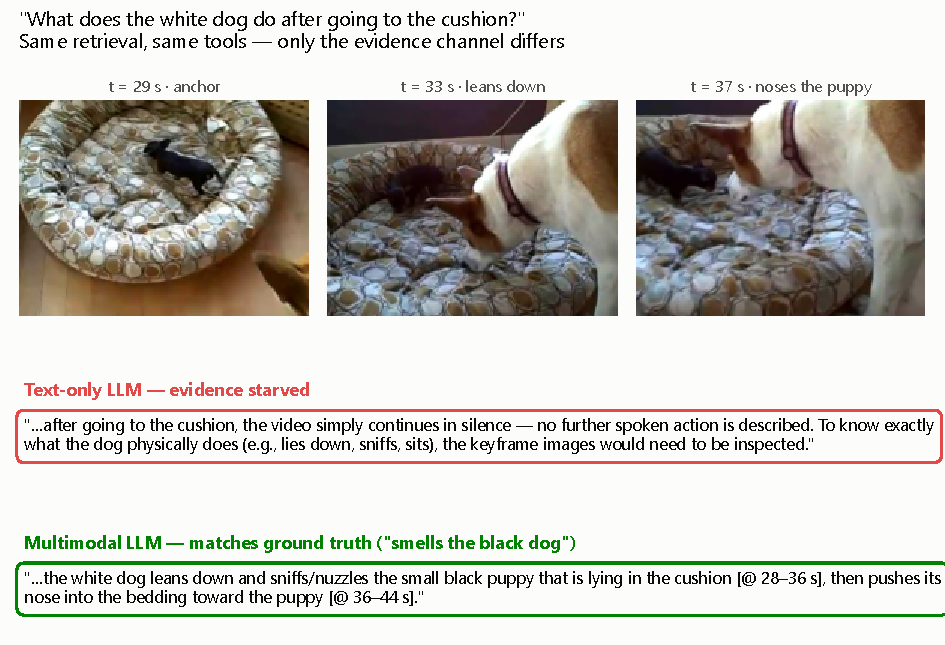
\includegraphics[width=0.96\linewidth,height=\textheight,keepaspectratio,alt={White-dog qualitative case: retrieved keyframes and answers under text-only and visual evidence.}]{../figures/fig8_whitedog_case.pdf}
\caption{White-dog qualitative case: retrieved keyframes and answers
under text-only and visual evidence.}
\end{figure}

\subsection{Prior-only baselines: what the .341 floor actually
was}

Two readings of the text-only TN floor deserve separation. Part of the
margin above random could reflect genuine transcript evidence; part
could reflect NExT-QA answer priors --- a language model can sometimes
reject implausible distractors without any evidence. To separate them,
both models answered the same 150 questions with \emph{no tool access at
all} --- the question and its five options, nothing else (Table 5.5,
prior-only rows; 150/150 completed each).

The result overturns the natural reading of the floor. Both models score
.560 overall without evidence --- coincidentally identical headlines
over different by-type profiles --- and the text-only model's own TN
prior is \textbf{.568}. The .341 text-only TN figure was therefore never
a floor: it is a \emph{suppression}. Given transcript-only evidence on
questions whose answers are visual, the same model performs .227
\textbf{below} its own prior (paired on the 44 TN questions: 14 flips
away from correct against 4 toward it; exact McNemar p = .031, bootstrap
95\% CI {[}−.409, −.045{]}). The mechanism is visible in the §5.4.1
transcripts: instructed to ground its answer in evidence, the model
dutifully reasons from segments that contain nothing relevant --- and
abandons the prior that would have served it better. When the channel
carries no signal for the question asked, delivered evidence is not
merely unhelpful; it is anti-informative.

The same accounting reframes the agent comparison. The simple agent's
.447 sits significantly below the bare prior (p = .024, CI {[}−.207,
−.020{]}); the graph agent's .547 recovers only to parity with it (p =
.88). And the recovery is not uniform but a sum of opposing type-level
effects: transcript evidence genuinely beats the prior where speech
describes the concurrent scene (TC .773 vs a .545 prior), is roughly
neutral on the causal types (CW .590 vs .574; CH .619 vs .524), and is
destructive on TN as above. Averaged over the type mix, the best
text-only stack lands where the bare model started.

Visual evidence is the only channel measured that beats the prior.
Within the multimodal model, the full stack adds +.167 over its own
prior (.560 \ensuremath{\rightarrow} .727; 37 flips up against 12 down;
exact McNemar p = .0005, CI {[}+.080, +.253{]}), and on TN the keyframe
evidence of §5.4.2 lifts its .455 prior to .636. Three consequences
follow. First, the .200 random floor is the wrong bar for
multiple-choice video QA --- the right bar is the bare model's prior,
and every absolute accuracy in this chapter should be calibrated against
.560. Second, the clean attributions are within-model, within-channel
pairs; comparisons across Table 5.5's rows conflate base-model strength,
evidence channel, and agent machinery. Third, grounding discipline has a
measurable cost when the channel is empty --- a design implication taken
up in §6.1.

\subsection{Best-configuration run and contextualisation with published
systems}

The strongest components identified across this chapter were finally
combined into one configuration: the SigLIP index (§5.3.4) with ViT-L
visual re-ranking inside the agent's search tool, the LangGraph agent
(§5.4.1), and the multimodal evidence channel (§5.4.2). On the same
150-question sample this configuration reaches \textbf{.727} overall
(Table 5.5, bottom row; 95\% CI {[}.655, .798{]}; zero failed runs;
approximately US\$25 of API usage). The gains concentrate where each
component predicts: causal questions reach .852 (CW) and .762 (CH) ---
the multimodal evidence lets the model \emph{see} the causes it
previously had to guess --- and TN rises from .341 to .568, confirming
§5.4.2's diagnosis while remaining the hardest type.

One result inside that figure runs against the trend and should be
stated rather than averaged away. On the same 44 TN items, under the
same multimodal evidence channel, the graph agent's .568 is \emph{three
questions below} the simple agent's .636 (§5.4.2): adding the temporal
tool and the reflection pass did not help here, and marginally hurt. At
n = 44 a three-question gap is well inside sampling noise and no claim
of a real regression is made. The direction is nonetheless consistent
with a structural gap in the current design --- the reflection node
audits a \emph{text} rendering of the gathered evidence, so on questions
whose answer is a silent visual action it interposes a text-mediated
check on a judgement the model made from keyframes, and has nothing to
contribute. This makes the keyframe-aware reflection pass the one
component interaction the dissertation leaves untested (§6.2), and the
headline TN figure for the evidence-channel effect remains §5.4.2's .636
under the simple agent.

To situate these numbers, Table 5.7 lists published zero-shot results on
the NExT-QA validation set alongside this system's, and the closest
published temporal grounding figures on NExT-GQA.

\textbf{Table 5.7 --- Contextualisation with published systems
(protocols differ; see caveats below).}

\begin{longtable}[]{@{}
  >{\raggedright\arraybackslash}p{(\linewidth - 4\tabcolsep) * \real{0.3333}}
  >{\raggedright\arraybackslash}p{(\linewidth - 4\tabcolsep) * \real{0.3333}}
  >{\raggedright\arraybackslash}p{(\linewidth - 4\tabcolsep) * \real{0.3333}}@{}}
\toprule\noalign{}
\begin{minipage}[b]{\linewidth}\raggedright
System
\end{minipage} & \begin{minipage}[b]{\linewidth}\raggedright
Protocol
\end{minipage} & \begin{minipage}[b]{\linewidth}\raggedright
NExT-QA val acc.
\end{minipage} \\
\midrule\noalign{}
\endhead
\bottomrule\noalign{}
\endlastfoot
Random & --- & .200 \\
SeViLA zero-shot \autocite{yu2023sevila} & full val, fine-tuned
localiser & approximately .636 \\
LLoVi \autocite{zhang2024llovi} & full val, GPT-based & approximately
.677 \\
VideoAgent \autocite{wang2024videoagent} & full val, GPT-4 + iterative
frame selection & .713 \\
\textbf{This work, best config} & grounded 150-q sample, ≤6
segments/search & \textbf{.727} {[}.655, .798{]} \\
\end{longtable}

\begin{longtable}[]{@{}
  >{\raggedright\arraybackslash}p{(\linewidth - 4\tabcolsep) * \real{0.3333}}
  >{\raggedright\arraybackslash}p{(\linewidth - 4\tabcolsep) * \real{0.3333}}
  >{\raggedright\arraybackslash}p{(\linewidth - 4\tabcolsep) * \real{0.3333}}@{}}
\toprule\noalign{}
\begin{minipage}[b]{\linewidth}\raggedright
Grounding
\end{minipage} & \begin{minipage}[b]{\linewidth}\raggedright
Protocol
\end{minipage} & \begin{minipage}[b]{\linewidth}\raggedright
metric
\end{minipage} \\
\midrule\noalign{}
\endhead
\bottomrule\noalign{}
\endlastfoot
FrozenBiLM (NG+) \autocite{xiao2024nextgqa} & NExT-GQA test, answer
grounding & mIoU .096 \\
Temp{[}CLIP{]} (NG+) \autocite{xiao2024nextgqa} & NExT-GQA test, answer
grounding & mIoU .121 \\
SeViLA \autocite{xiao2024nextgqa} & NExT-GQA test, answer grounding &
mIoU .217 \\
\textbf{This work, SigLIP + decomposition} & NExT-GQA val, top-1
retrieved segment & tIoU@1 \textbf{.230} \\
\end{longtable}

Three caveats govern the reading of Table 5.7, and are repeated wherever
these numbers are cited. First, the QA comparison is \emph{indicative,
not a leaderboard claim}: published systems evaluate the full
approximately 5,000-question validation set while the figure here comes
from a 150-question sample of the grounded subset, so the honest
statement is that the best configuration performs \emph{at, and in point
estimate above, the published zero-shot state of the art on this
sample}, with a confidence interval that overlaps the strongest
published figure. Second, the comparison is not equal-resource: this
system answers from at most six retrieved segments per search under
approximately US\$0.17 per question, but benefits from a stronger
underlying LLM (claude-opus-4-8) than the GPT-4-era published systems
--- LLM generation and method both differ, and this chapter's internal
ablations (not Table 5.7) are what isolate the method's contribution.
The prior-only baseline (§5.4.3) quantifies the model-strength component
directly: claude-opus-4-8 reaches .560 on these questions with no tools
at all, so the honest within-model attribution for the method is .560
\ensuremath{\rightarrow} .727 (+.167, p = .0005). Third, the grounding
rows compare related but non-identical protocols (their mIoU grounds a
QA model's answer on the test split; tIoU@1 here scores the top
retrieved segment on val); they are included because both measure
``where the system points for its evidence'', where this retrieval-first
design proves competitive with --- and in point estimate above ---
published weakly-supervised grounding, while additionally emitting the
citation as a first-class output.

\section{Cross-domain replication: speech-dense
video}

The causal analyses of §5.2 and §5.3.1 blame the text channel's failure
on a property of the \emph{domain} rather than of the components:
NExT-QA's home videos are speech-sparse, 60\% of segments carrying any
speech and much of that multilingual chatter. That reading makes a
falsifiable prediction --- in a speech-dense, single-language domain the
same components should reverse sign --- and this section tests it
directly.

\textbf{Setup.} Forty validation videos of YouCook2
\autocite{zhou2018youcook2}, which is English-narrated cooking
instruction of mean duration approximately 5 minutes, were ingested by
the \emph{unchanged} pipeline: the same 8 s / 4 s segmentation, the same
Whisper transcription, and the same ViT-B-32 index as the §5.2 baseline,
producing 3,110 visual and 3,100 transcript vectors over 3,173 segments.
The benchmark's own step annotations serve as queries. Each annotated
step (a sentence plus a ground-truth {[}start, end{]} interval) becomes
one moment-retrieval query, 314 in total, scored under the §5.1
protocol. The speech-density contrast is stark: 97.7\% of segments carry
speech (3,100 of 3,173, against 60\% on NExT-QA), and the speech is
task-aligned narration rather than incidental conversation.

\textbf{Table 5.8 --- Modality comparison on YouCook2 (ViT-B-32 index, τ
= 0.5, 314 step queries).}

\begin{longtable}[]{@{}lllllll@{}}
\toprule\noalign{}
Scope & Modality & R@1 & R@5 & R@10 & MRR & tIoU@1 \\
\midrule\noalign{}
\endhead
\bottomrule\noalign{}
\endlastfoot
corpus & visual & .048 & .099 & .143 & .076 & .058 \\
corpus & text & .096 & .213 & .261 & .145 & .128 \\
corpus & fused (α=.5) & .099 & .197 & .287 & .145 & .108 \\
video & visual & .115 & .245 & .318 & .173 & .152 \\
video & text & .146 & .331 & .392 & .221 & .199 \\
video & fused (α=.5) & .169 & .350 & .420 & .247 & .215 \\
\end{longtable}

Every sign flips as predicted. Transcript retrieval \textbf{doubles}
visual retrieval in corpus scope (R@1 .096 vs .048; MRR .145 vs .076)
--- the mirror image of §5.2, where visual led text by an order of
magnitude. Late fusion, which on NExT-QA never beat visual-only at any
weight (§5.3.1), is here the \emph{best configuration in video scope on
every metric} (MRR .247 against .221 text-only and .173 visual-only) and
the best deep-rank configuration in corpus scope (R@10 .287). The α
sweep confirms the direction of the regime: quality now \emph{falls} as
the visual weight rises (corpus R@10 .287 at α = .5
\ensuremath{\rightarrow} .194 at α = .8), where on NExT-QA the same
sweep improved monotonically toward visual. The ordering is unchanged at
the looser τ = 0.3 (corpus text R@1 .191 vs visual .099).

The replication turns the conditionality \emph{claim} of §5.3.1 into a
measured result: those negative results are properties of the domain,
not of the components.

Part of the reversal, however, is \emph{register} rather than speech
density. YouCook2 queries are step descriptions phrased in the
narrator's own vocabulary, where NExT-QA questions are causal
reformulations of silent visual events. The two factors move together in
this design and it cannot separate them; doing so would need a third
condition, speech-dense video queried out of register, which was not
run. What the replication does establish is the weaker but sufficient
claim: with every component held fixed, changing the domain reverses the
ordering, so that ordering is not a property of the components. The
practical corollary is a \emph{domain-adaptive} modality policy,
weighting the transcript channel by measured speech density and register
match with exactly this harness, rather than a fixed design choice.

Two qualifications temper the result. The second corpus is small (40
videos, sized to the remaining project budget), and the replication
covers the retrieval layer only, since the QA-stage experiments of §5.4
were not repeated. The direction and magnitude of the reversals (2× on
corpus R@1, fusion best across the board in video scope) are nonetheless
far outside plausible noise for a deterministic 314-query evaluation.

\section{System-level measurements}

The offline stage processed all 567 videos in approximately 2 h on a
single RTX 4050 laptop GPU (6 GB): keyframe extraction at \textless1 s
per video and Whisper large-v3 (int8, CTranslate2) transcription at
2--20 s per video; CLIP ViT-B-32 embedding and indexing of 5,725
segments adds approximately 15 min, and the SigLIP index approximately
35 min. The resulting index is portable (17 MB of vectors per backbone
in npz form plus the ChromaDB store) and queries run interactively:
question encoding is sub-second on GPU, HNSW search over 5,725 vectors
is milliseconds, and the visual re-ranker adds one batched matrix
product over 30 candidates. End-to-end agent answers complete in 15--60
s depending on tool rounds, dominated by LLM latency. Marginal API costs
are small: query decomposition for the entire split cost approximately
US\$0.15 (cached thereafter), a 150-question text-only QA run
approximately US\$0.35, and the 44-question multimodal run approximately
US\$3. The retrieval programme and the text-only QA studies --- every
experiment of §5.2, §5.3 and §5.5, plus the agent comparison of §5.4.1
--- are therefore reproducible on one consumer laptop plus approximately
US\$5 of API usage. The one expensive run is the 150-question multimodal
best configuration of §5.4.4, at approximately US\$25 (approximately
US\$0.17 per question, dominated by keyframe image tokens), bringing the
full chapter to approximately US\$30 end to end.

\section{Summary}

\textbf{RQ1.} Visual retrieval outperforms the text-only baseline by an
order of magnitude in corpus scope, and the corpus/video gap identifies
cross-video confusion, not within-video imprecision, as the dominant
error mode.

\textbf{RQ2.} Five ablation results answer the embedding-strategy
question. (i) Naive late fusion cannot rescue a weak text channel at any
weight. (ii) Query decomposition buys recall at depth while visual
re-ranking buys top-rank precision, and the two compose. (iii) SigLIP is
the strongest index backbone, nearly doubling baseline R@1. (iv) A
two-stage cheap-index/expensive-re-rank design matches the expensive
index outright. (v) The modality ordering itself is domain-conditional:
on YouCook2 (§5.5) transcript retrieval doubles visual retrieval and
late fusion becomes the best configuration, exactly as the causal
analysis predicted.

\textbf{RQ3.} A LangGraph agent with temporal tools and self-reflection
improves QA accuracy by 10 points over a single-loop agent (McNemar p =
.031), and a controlled evidence-channel experiment shows visual
evidence nearly doubling temporal-next accuracy (p = .004). Modality
therefore matters at the answering stage independently of retrieval.

\textbf{Calibration.} Prior-only baselines reframe every QA number
above. Both models score .560 with no evidence at all. The best
text-only stack merely matches that prior, and on temporal-next
questions falls .227 below it (p = .031), while the multimodal stack
exceeds its own prior by +.167 (p = .0005). Visual evidence is the only
channel measured that beats the bare model.

Combining the best-measured component in every slot yields .727 five-way
accuracy --- at, and in point estimate above, the published zero-shot
state of the art on this sample --- while temporal grounding proves
competitive with published weakly-supervised answer-grounding methods
under a stricter, citation-producing protocol. Chapter 6 discusses the
limitations and generality of these findings.
